\documentclass{article}
\usepackage[utf8]{inputenc}
\usepackage{hyperref}
\usepackage{mathtools}
\usepackage{graphicx}

\title{DT057A Project}
\author{raho1501 \& majo1412 \& mafl1400}
\date{May 2019}

\begin{document}

\maketitle

\section{Part I: PRNG and Random Variables}
\begin{enumerate}
  \item A LCG random generator was created in a file named "lcg.h" for generating random uniformed numbers. The file can be found in the git repo.
  \item 1000 values were generated and transformed onto the range [0,1] by calling the function "norm\_gen()" in the "lcg.h" header. A bulk function was also created if the 1000 values were in an array, then the GPU accelerated function "transformKernel(*input, mod, output,1000)" was called, which can be found in the header "func.cuh".
  \item Our function was compared with the ns3 implementation and the result was that our implementation was worse. Ours were cyclic while the ns-3 wasn't as obviously-cyclic.
  \item The ns3 UniformRandomVariable does not seem to repeat and uses more values between 0 and 1. Using our implementation with the values seed=1, a=13, c=1 and m=100 creates a cycle with 20 values before repetition. Both are however uniformally distributed. Using a m that is a large prime would mean that we get as many values as possible between 0 and the large prime this is because p \% n != 0 for any prime p and value n < p. Howerer if a and p are coprime then this also results in a simmilar way to using primes as m. So if we want to make the modulo operation as effective as possible we can choose a m that is a power of 2. Then if we choose an odd value as a, a and m are coprime.
  \item Combined Multiple-Recursive Generator. The normal random variable in ns3 uses the polar form of the Box-Muller method which is a rejection sampeling method that aviods using trigometric functions. \url{https://en.wikipedia.org/wiki/Box\%E2\%80\%93Muller_transform}
  \item Our implementation is faster we get a time of 3.320s for ns3 it takes 3.806s. We tested with 10 million generated values. With 1 billion generated values our takes ~18.468s while ns3 takes ~1m 7.544s
  \item Acording to the lectures we can use inverse cdf to function on the generated uniform random variable to create a random variable following the desired distriobution. For exponential distrobution we can use the function:$$ F^{-1}_x(u)) = \frac{-1}{\beta} * ln(1-u) \implies x \in \exp{(\lambda)} $$
  \item When comparing our implementation with the ns3 implementation we get quite simmilar distributions. However our implementation seems have a bit less variance than the ns3 version.
\end{enumerate}
\section{Part II: Mathematical Modelling of a system of Queues}
\begin{figure}[h!]
  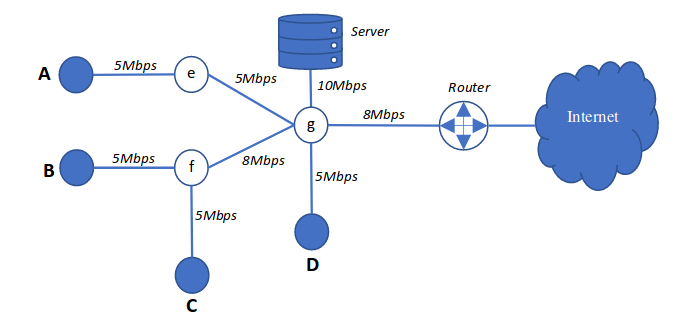
\includegraphics[width=\linewidth]{netmap.png}
  \caption{Network topology}
  \label{fig:netmap}
\end{figure}
By inspecting the figure \ref{fig:netmap} we made a Kleinrock approximation to calculate the average number of packets in the system.
\begin{table}[h]
\centering
\label{Arrivalrates}
\caption{Arrival rates}
\begin{tabular}{|l|l|l|}
\hline
$\lambda_{ij}$ & Calculation & Arrival rate (Packets/s) \\ \hline
$\lambda_{ae}$ & $\frac{1}{2ms}$  & 500 \\ \hline
$\lambda_{bf}$ & $\frac{1}{2ms}$  & 500 \\ \hline
$\lambda_{cf}$ & $\frac{1}{0.5ms}$  & 2000 \\ \hline
$\lambda_{dg}$ & $\frac{1}{1ms}$  & 1000 \\ \hline
$\lambda_{fg}$ & $\lambda_{bf} + \lambda_{cf}$  & 2500  \\ \hline
$\lambda_{eg}$ & $\lambda_{ae}$ & 500 \\ \hline
$\lambda_{gs}$ & $\lambda_{fg} + \lambda_{dg} + \lambda_{eg}$ & 4000 \\ \hline
\end{tabular}
\end{table}
After the arrival rates had been calculated the service rates were calculated.
\begin{table}[h]
\centering
\label{departurerates}
\caption{Departure rates}
\begin{tabular}{|l|l|}
\hline
$\mu_{ij}$ & Service rate(Packets/s)\\ \hline
$\mu_{ae}$ & 6250 \\ \hline
$\mu_{eg}$ & 6250 \\ \hline
$\mu_{bf}$ & 6250 \\ \hline
$\mu_{cf}$ & 6250 \\ \hline
$\mu_{dg}$ & 6250 \\ \hline
$\mu_{fg}$ & 10000 \\ \hline
$\mu_{gs}$ & 12500 \\ \hline
\end{tabular}
\end{table}
These were then used to calculate the average number of packets in each line according to the formula:
$$N_{ij} = \frac{\lambda_{ij}}{\mu_{ij} - \lambda_{ij} }$$
Which when calculated using the aquired values becomes:
$$N_{ae} = \frac{\lambda_{ae}}{\mu_{ae} - \lambda_{ae} } \implies \frac{500}{6250 - 500 } = 0.0869565 $$
$$N_{eg} = \frac{\lambda_{eg}}{\mu_{eg} - \lambda_{eg} } \implies \frac{500}{6250 - 500 } = 0.0869565 $$
$$N_{bf} = \frac{\lambda_{bf}}{\mu_{bf} - \lambda_{bf} } \implies \frac{500}{6250 - 500 } = 0.0869565 $$
$$N_{cf} = \frac{\lambda_{cf}}{\mu_{cf} - \lambda_{cf} } \implies \frac{2000}{6250 - 2000 } = 0.470588 $$
$$N_{dg} = \frac{\lambda_{dg}}{\mu_{dg} - \lambda_{dg} } \implies \frac{1000}{6250 - 1000 } = 0.190476 $$
$$N_{fg} = \frac{\lambda_{fg}}{\mu_{fg} - \lambda_{fg} } \implies \frac{2500}{10000 - 2500 } = 0.333333 $$
$$N_{gs} = \frac{\lambda_{gs}}{\mu_{gs} - \lambda_{gs} } \implies \frac{4000}{12500 - 4000 } = 0.470588 $$
$$Equations 1. Individual number of packets.$$

Which then is used to calculate the average number of packets in the whole system using the formula:
$$ \overline{N} = \sum N_{ij} $$
Which gives us a number of:
$$ \overline{N} = \sum N_{ij} = \frac{500}{6250 - 500 } + \frac{500}{6250 - 500 } + \frac{500}{6250 - 500 } + \frac{2000}{6250 - 2000 } + $$ 
$$ \frac{1000}{6250 - 1000 } + \frac{2500}{10000 - 2500 } + \frac{4000}{12500 - 4000 } = 1.638898 packets $$ 


Which concludes the section with the answers to the questions. The average number of packets are 1.638898 packets and the number of packets per link can be found in equations 1.


\section{Part III: Simulations and Results Comparison}

\end{document}
